\subsection{Постановка задачи}

Инструмент должен решать задачу тестирования распределенной системы, внутри которой исполняется код студента.

Распределенную систему мы представим в виде набора узлов, объединенных в общую сеть. Узлы могут коммуницировать друг с другом только с помощью отправки сообщений.

Сеть мы считаем асинхронной и недетерминированной – она может произвольно задерживать и переупорядочивать отправляемые узлами сообщения. Если система будет корректно работать в асинхронной сети, то и в реальной, частично синхронной сети тоже.

Внутри узла исполняются недетерминированные программы. Также узлы могут отказывать, то есть перезагружаться в произвольные моменты и/или навсегда отключаться.

Мы считаем, что набор узлов системы реализует некоторый распределенный сервис, с которым клиенты взаимодействуют через протокол RPC. 

Клиенты тоже являются узлами сети. 

Они посылают системе запросы и получают ответы, в результате возникает конкурентная история, состоящая из отрезков запросов (рис.~\ref{fig:history_example}). Свойства системы формулируются как утверждения про допустимые истории, которые может порождать система.

\begin{figure}[h]
    \centering
    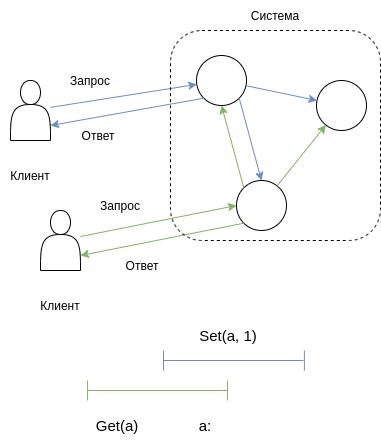
\includegraphics[width=0.5\textwidth]{img/task.png}
    \caption{Пример истории запросов}
    \label{fig:history_example}
\end{figure}

В данной работе нас прежде всего интересует задача репликации, так что распределенный сервис  представляет собой хранилище данных с операциями Set и Get, а свойство, которое мы ожидаем от системы – модель согласованности \cite{consistency}, в первую очередь – линеаризуемость \cite{linearizability}.

Наконец, сформулируем задачу – по реализации узлов системы проверить выполнение заявленных свойств независимо от поведения сети между узлами, часов и т.д.
